\documentclass[11pt]{amsart}
\usepackage{amsmath,amssymb,amsthm,mathtools}
\usepackage{thmtools}
\usepackage{cleveref}
\usepackage{mathdots}
\newtheorem{theorem}{Theorem}[section]
\newtheorem{proposition}[theorem]{Proposition}
\newtheorem{lemma}[theorem]{Lemma}
\newtheorem{corollary}[theorem]{Corollary}
\newtheorem{algorithm}[theorem]{Algorithm}
\theoremstyle{definition}
\newtheorem*{definition}{Definition}
\newtheorem*{example}{Example}
\theoremstyle{remark}
\newtheorem*{remark}{Remark}
\newcommand{\F}{\mathbb F}
\newcommand{\Z}{\mathbb Z}
\newcommand{\N}{\mathbb N}
\usepackage{tikz}
\DeclareMathOperator{\Col}{Col}
\DeclareMathOperator{\Diag}{Diag}

\begin{document}

\subsection{The optimization problem}
We unwind the definitions involved in the problem more explicitly now.

\subsubsection{Notation for base-$q$ digits}
For each $k_i$, we let $a_{i,n}$ denote its base-$q$ digits
\[ k_i = \sum_{n\geq 0}a_{i,n}q^n, \qquad 0\leq a_{i,n}\leq q-1.  \]
For $k$ itself, we use $C_n$ for its base-$q$ digits,
\[ k = \sum_{n \ge 0} C_n q^n, \qquad 0 \le C_n \le q-1. \]
For convenience, $a_{i,n} = 0$ if $n < 0$.

\subsubsection{Admissible decompositions}
We will say a decomposition
\[ k=k_0+k_1q+\cdots+k_dq^d \]
is \emph{admissible} if $k_0+\cdots+k_d$ is carry-free in base-$q$.

We can visualize the hypotheses by drawing the grid shown in \Cref{fig:addition_table}.
This is a grid which is infinite to the left,
with columns \dots, $\Col_2$, $\Col_1$, $\Col_0$, with $d+1$ rows.
In the $i$\textsuperscript{th} row of $\Col_m$ we imagine placing $a_{i,m-i}$ stones.
\begin{figure}[ht]
  \centering
  \[
    \begin{array}{cc|cccccccc}
      && \dots & \Col_{d} & \Col_{d-1} & \dots & \Col_3 & \Col_2 & \Col_1 & \Col_0 \\ \hline
      \text{Row $0$} & k_0 & \dots & a_{0,d} & a_{0,d-1} & \dots & a_{0,3} & a_{0,2} & a_{0,1} & a_{0,0} \\
      \text{Row $1$} & q k_1 & \dots & a_{1,d-1} & a_{1,d-2} & \dots & a_{1,2} & a_{1,1} & a_{1,0} \\
      \text{Row $2$} & q^2 k_2 & \dots & a_{2,d-2} & a_{2,d-3} & \dots & a_{2,1} & a_{2,0} \\
      \text{Row $3$} & q^3 k_3 & \dots & a_{3,d-3} & a_{3,d-4} & \dots & a_{3,0} \\
      \multicolumn{1}{c}{\vdots} & \vdots & \dots & \vdots & \vdots & \iddots \\
      \text{Row $d-1$} & q^{d-1} k_{d-1} & \dots & a_{d-1,1} & a_{d-1,0} \\
      \text{Row $d$} & q^d k_d & \dots & a_{d,0} \\ \hline
      \text{Sum} & k & \dots & C_d & C_{d-1} & \dots & C_3 & C_2 & C_1 & C_0
    \end{array}
  \]
  \caption{Admissible decompositions, drawn as an addition table in base-$q$.
    We imagine placing $a_{i,m-i}$ stones in the $i$\textsuperscript{th} row of $\Col_m$.}
  \label{fig:addition_table}
\end{figure}

A decomposition corresponds to a way of filling in the digits in
\Cref{fig:addition_table} such that both of the following
capacity constraints hold:
\begin{description}
  \item[Column capacity] We require that summing the addition table in \Cref{fig:addition_table}
    indeed gives
    \[ \sum q^i k_i = \sum C_n q^n. \]

    One would expect \emph{a priori} that there could be some base-$q$ carrying.
    However, \Cref{lem:H1-carry-elimination} will show this case never produces
    optimal values.
    Thus we can regard this condition as saying $\Col_m$ has exactly $C_m$ stones.

  \item[Diagonal capacity]
    For each $n$, let $\Diag_n$ denote the cells labeled $a_{i,n}$ for $0 \le i \le d$.
    Then for every $n$, admissibility requires that
    \begin{equation} \label{eq:source-capacity-H1}
      \text{number of stones in } \Diag_n = \sum_{i=0}^d a_{i,n} \leq q-1.
    \end{equation}
\end{description}

\subsubsection{The objective function $\Phi$}
We see that we are trying to minimize
\begin{align*}
  -\sum_{i=0}^d k_i b(i,d)
  &=\sum_{i=0}^d k_i\left(\frac{q^{d+1}-q^{i+1}}{q-1}+iq^i\right)
  =\frac{q^{d+1}}{q-1}\sum_{i=0}^d k_i
    -\frac{q}{q-1}\sum_{i=0}^d k_iq^i+
     \sum_{i=0}^d iq^ik_i\\
  &=\frac{1}{q-1}
  \left( q^{d+1}\sum_{i=0}^d k_i+(q-1)\sum_{i=0}^d iq^ik_i \right)
  -\frac{qk}{q-1}.
\end{align*}
The final term is fixed once $k$ is fixed.
Hence, if we define
\begin{equation}\label{eq:Phi-H1}
  \begin{aligned}
    g_i &\coloneq q^{d+1-i} + (q-1) \cdot i \\
    \Phi(k_0,\ldots,k_d) &\coloneq q^{d+1}\sum_{i=0}^d k_i+(q-1)\sum_{i=0}^d iq^ik_i
    = \sum_{i,n} q^{n+i} g_i \cdot a_{i,n}
  \end{aligned}
\end{equation}
then the problem is equivalent to the following proposition:
\begin{proposition}\label{prop:H1-optimization}
  Let $q=p$, $d\geq 0$, and $k\geq 0$ be fixed.
  Among all admissible decompositions, there is a unique one minimizing $\Phi$
  as defined in \eqref{eq:Phi-H1}.
\end{proposition}
In words, the objective function $\Phi$
is obtained by assigning a weight $q^{n+i} g_i$ to each stone
in the cell labeled $a_{i,n}$ and summing.
We remark that, since $g_i-g_{i+1}=(q-1)(q^{d-i}-1)>0$, the $g_i$ are decreasing:
\begin{equation}\label{eq:g-decreasing-H1}
  g_0>g_1>\cdots>g_d.
\end{equation}

The proof has two parts.
First we show that a minimizer has no carries in the addition table in \Cref{fig:addition_table}.
Then the problem becomes a transparent assignment problem for the individual base-$q$ digit units of $k$.

\subsection{No shifted carries in \Cref{fig:addition_table}}
The next lemma is the first decisive simplification.
\begin{lemma}\label{lem:H1-carry-elimination}
  If $(k_0,\ldots,k_d)$ is an admissible decomposition minimizing $\Phi$, then
  \[ \sum a_{i,m-i} \leq q-1\qquad\text{for every }m.  \]
  Equivalently, $\Col_m$ of \Cref{fig:addition_table} has exactly $C_m$ stones.
\end{lemma}
\begin{proof}
Assume for contradiction that a minimizing admissible decomposition has a carry,
first occurring in $\Col_m$.
We perform the following change:
\begin{itemize}
  \item Choose any $q$ stones in $\Col_m$ and remove them.
  \item Among the rows occupied by these chosen stones,
    let $j$ be maximal subject to $j<d$
    (since $a_{d,m-d} < q$, not all stones are in the final row).
    Add one stone to $a_{j+1,m-j}$.
\end{itemize}
The addition table in \Cref{fig:addition_table} remains valid,
since we removed a total of $q$ stones from $\Col_m$ and added one to $\Col_{m+1}$.
Moreover, the newly added stone was in $\Diag_{m-j}$,
which had at least one stone removed;
hence the diagonal capacity constraints are still satisfied too.

It remains to compare the values of $\Phi$.
The removed stones contribute
\[
  q^m\sum_{\text{chosen}}g_i,
\]
while the inserted stone contributes
\[
  q^{m+1}g_{j+1}=q^m qg_{j+1}.
\]
Hence the replacement lowers $\Phi$ if
\begin{equation}\label{eq:H1-Phi-ineq}
  \sum_{\text{chosen}}g_i > qg_{j+1}.
\end{equation}
Recall from \eqref{eq:g-decreasing-H1} that $g_i$ are decreasing.
By the definition of $j$, all stones appear in either row $d$ or rows $\le j$.
Row $d$ contains $a_{d,m-d} \le q-1$ stones, so
\[ \sum_{\text{chosen}}g_i \ge  g_j+(q-1)g_d.  \]
A direct calculation gives
\begin{align*}
  g_j+(q-1)g_d-qg_{j+1}
  &=\bigl(q^{d+1-j}+(q-1)j\bigr)
    +(q-1)\bigl(q+(q-1)d\bigr)\\
  &\qquad -q\bigl(q^{d-j}+(q-1)(j+1)\bigr)\\
  &=(q-1)^2(d-j)>0.
\end{align*}
Thus the replacement strictly lowers $\Phi$, contradicting minimality.
Therefore no shifted carry can occur in a minimizer.
\end{proof}

\subsection{The assignment problem and its greedy solution}
Thanks to \Cref{lem:H1-carry-elimination},
we can now regard \Cref{fig:addition_table} as a totally combinatorial problem
where $\Col_m$ has exactly $C_m$ stones
and $\Diag_n$ has at most $q-1$ stones,
and we wish to minimize a sum of weights across all the stones.

We can now describe the greedy algorithm concretely and simply:
\begin{algorithm}
  \label{alg:H1-greedy}
  Allocate the stones of $\Col_0$, $\Col_1$, \dots, in that order.
  For the $m$\textsuperscript{th} column ($m \ge 0$), we place each of the $C_m$ stones in $\Col_m$
  (one at a time) in the lowest cell that stone can be placed
  in without violating diagonal capacity constraints.
\end{algorithm}

\begin{example}
  Let $q = 11$, $d = 3$, and $k = 8675309_{11}$ (in base eleven).
  Then the diagonal constraint is that each diagonal has at most $10$ stones in it.
  The corresponding greedy output is:
  \[
    \begin{array}{c|ccc cccc}
      & \Col_6 & \Col_5 & \Col_4 & \Col_3 & \Col_2 & \Col_1 & \Col_0 \\ \hline
      \text{Row $0$} & 0 & 0 & 0 & 0 & 0 & 0 & 9 \\
      \text{Row $1$} & 0 & 0 & 0 & 0 & 2 & 0 \\
      \text{Row $2$} & 0 & 0 & 4 & 5 & 1 \\
      \text{Row $3$} & 8 & 6 & 3 & 0 \\ \hline
      k & 8 & 6 & 7 & 5 & 3 & 0 & 9
    \end{array}
  \]
\end{example}

\begin{lemma}
  The greedy assignment described in \Cref{alg:H1-greedy} minimizes $\Phi$.
\end{lemma}
\begin{proof}
  Let $a_{i,n}$ be the allocation minimizing $\Phi$.
  assume for contradiction it doesn't match the greedy allocation,
  and let $\Col_m$ be the rightmost column where they don't match.
  Choose the largest $j$ such that $a_{j,m-j}$ has fewer stones than the greedy allocation;
  then there exists some $i < j$ such that $a_{i,m-i} > 0$.
  We consider two cases:
  \begin{itemize}
  \item Suppose $\Diag_{m-j}$ is not at full capacity.
  Then we are free to move a stone directly downwards from $a_{i,m-i}$ to $a_{j,m-j}$.
  This changes the value of $\Phi$ by
  \[ q^{m} (g_j - g_i) < 0 \]
  due to \eqref{eq:g-decreasing-H1}, contradicting minimality.

  \item Suppose $\Diag_{m-j}$ is at full capacity already.
  This implies the existence of a $t > 0$ such that $a_{j+t,m-j} > 0$.
  Thus, we arrive at a picture like in \Cref{fig:parallelogram}.

  \begin{figure}[b]
    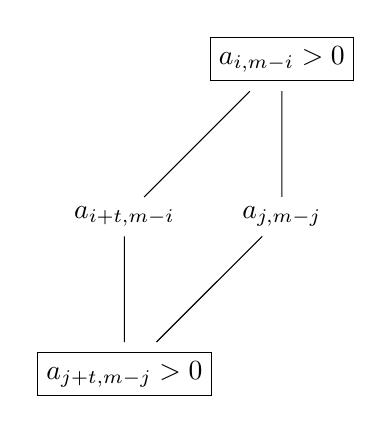
\begin{tikzpicture}[scale=2]
      \node (A) at (1,2)  {$\boxed{a_{i,m-i} > 0}$};
      \node (B) at (0,1)  {$a_{i+t, m-i}$};
      \node (C) at (0,0)  {$\boxed{a_{j+t, m-j} > 0}$};
      \node (D) at (1,1)  {$a_{j,m-j}$};
      \draw (A) -- (B) -- (C) -- (D) -- (A);
    \end{tikzpicture}
    \caption{An impossible parallelogram that we show can't appear in an optimal solution.}
    \label{fig:parallelogram}
  \end{figure}

  However, we prove that \Cref{fig:parallelogram} violates minimality by moving two stones:
  we remove one stone from each of $a_{i,m-i}$ and $a_{j+t,m-j}$
  and add one stone to $a_{i+t,m-i}$ and $a_{j,m-j}$ instead.
  This has no effect on column or diagonal sums, but it changes the value of $\Phi$ by
  \begin{align*}
    q^{m} (g_j - g_i) - q^{m+t} (g_{j+t}-g_{i+t})
    &= q^m \left[ (q^{d+1-j} - q^{d+1-i}) + (q-1)(j-i) \right] \\
    &\qquad - q^{m+t} \left[ (q^{d+1-(j+t)} - q^{d+1-(i+t)}) + (q-1)(j-i) \right] \\
    &= (q-1)(j-i)(q^m-q^{m+t}) < 0. \qedhere
  \end{align*}
  \end{itemize}
\end{proof}

\end{document}